\documentclass{amznotes}
\usepackage{pdfpages}
\usepackage{ctex}
\usepackage{float}
\usepackage{caption}
\usepackage{enumitem}
\usepackage{booktabs}
\usepackage{tabularx}
\usepackage{tikz}
\usepackage[svgnames]{xcolor}
\usetikzlibrary{mindmap,trees,shadows,positioning, arrows.meta}
% \usepackage{amssymb}     % 提供 \checkmark
\usepackage{lipsum}     % filler text
\newamzbox{rsbox}{结果}{result}{amztecboxcolor}
\newamzbox{ffbox}{方法}{way}{amzexboxcolor}
\newamzbox{jqbox}{渠道}{jq}{amznoteboxcolor}
\begin{document}
    \setlength{\parindent}{2em}
    
\includepdf[pages={1}]{./source/cover1.pdf}
    \setcounter{tocdepth}{1}
    \tableofcontents
    \newpage
    \chapter{假新闻的识别和应对}
\section{假新闻的类型}
\begin{enumerate}
  \item 图片与视频造假

  虚假的描绘以色列与哈马斯战争的场景的照片。
  \begin{figure}[H]
    \centering
    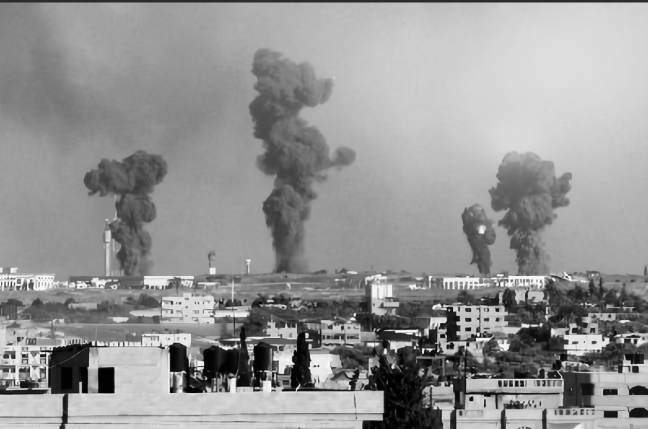
\includegraphics[width=.7\textwidth]{figures/假新闻/哈马斯.png}
    \caption{虚假战争的场景}
  \end{figure}
  \item 数据谣言

  生物学家刻意使用小样本容量,随机提供数据,只塑造关键信息,得出黑巧克力能帮忙减肥的结论。
  \begin{figure}[H]
    \centering
    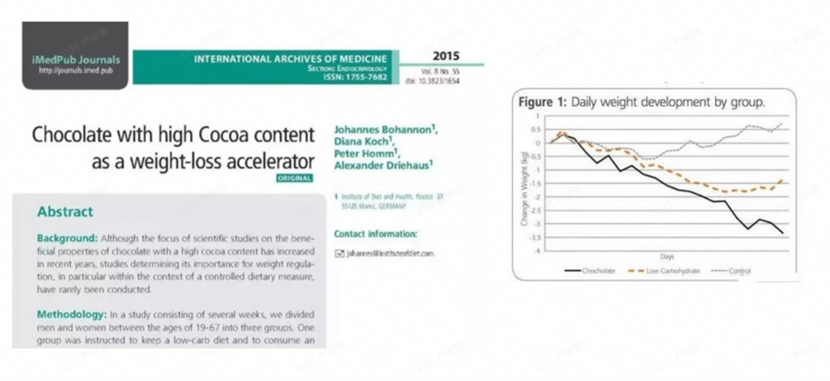
\includegraphics[width=.7\textwidth]{figures/假新闻/减肥.png}
    \caption{数据谣言}
  \end{figure}

  \item 引用作假

  通过引用所谓业内人士来作假,例如太阳报报道女王暗示支持脱欧,然而王室成员不能有任何政治倾向。
  \begin{figure}[H]
    \centering
    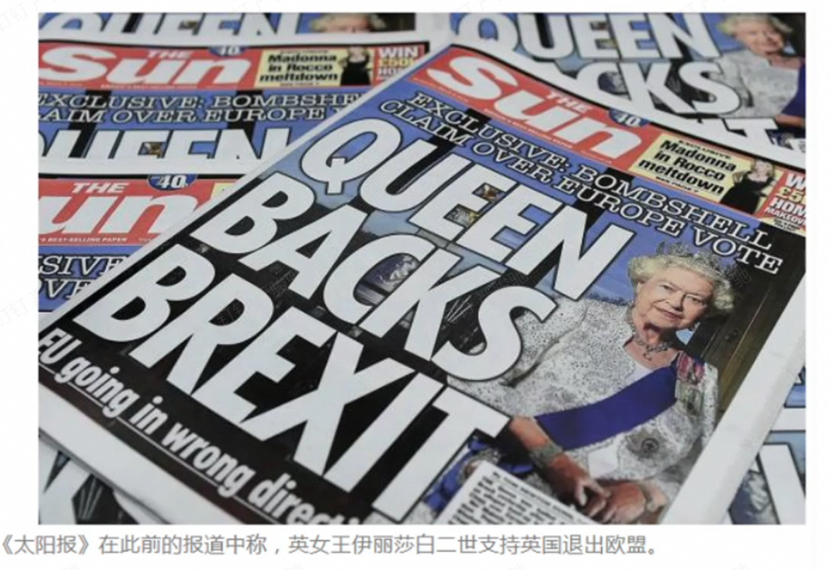
\includegraphics[width=.7\textwidth]{figures/假新闻/引用造假.png}
    \caption{引用造假}
  \end{figure}

  \item 真实的谎言

  \begin{dfnbox}{真实的谣言}{真实的谣言}
    内容大部分真实,然而在报道过程中利用模糊用词,刻意转换理解角度等手段使新闻符合读者预期
  \end{dfnbox}
  例如
  \begin{enumerate}
    \item 巴黎圣母院被大火烧毁+中国建筑师巴黎圣母院建筑竞赛夺冠$\ne$中国建筑师的这个设计方案,将会成为巴黎圣母院的重建方案。
    \item 英国的一个患癌男子感染新冠以后肿瘤消失$\ne$新冠能治愈肿瘤。
  \end{enumerate}

  \item 智能新闻
  \begin{dfnbox}{智能新闻}{智能新闻}
    完全利用AI智能生成,没有真实性
  \end{dfnbox}
\end{enumerate}
\section{假新闻泛滥的原因和危害}
\subsection{泛滥原因}
\begin{enumerate}
  \item 传播环境的影响
  \item 专业媒体竞争压力导致对核实和审查的忽视
  \item 受众的认知局限和心理特征
  \item 人工智能对虚假信息的重构
\end{enumerate}
\subsection{危害影响}
\begin{enumerate}
  \item 给当事人带来困扰,影响读者情绪和思维
  \item 影响新闻媒体公信力
  \item 社会秩序遭到破坏
  \item 影响国家形象
\end{enumerate}
\section{媒介素养与假新闻识别方法}
\begin{figure}[H]
  \centering
  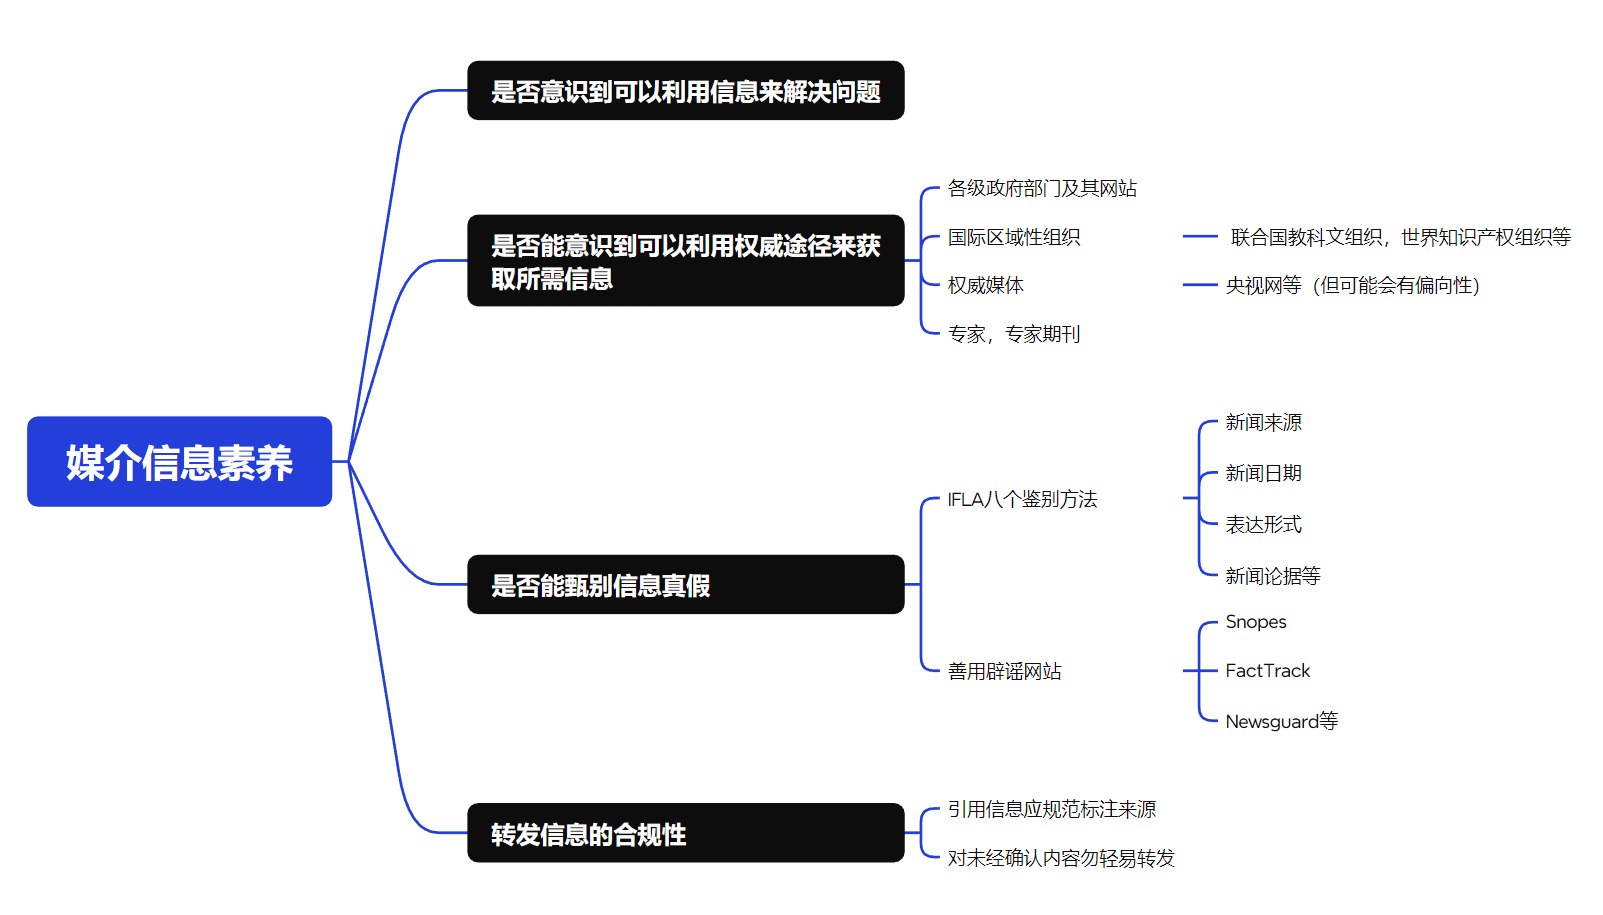
\includegraphics[width=\textwidth]{./figures/假新闻/思维导图.png}
  \caption{假新闻的应对方法}
\end{figure}
\chapter{科研}
\section{理工类文献检索方法}\label{数据库}
\subsection{数据库选择}

\subsubsection{中文数据库}

\begin{enumerate}
  \item \textbf{中国知网(CNKI):} 综合性数据库,涵盖期刊、学位论文、会议论文、专利等多种文献类型,是学位论文检索的首选之一。
  \item \textbf{万方数据:} 综合性数据库,资源丰富,包含期刊、学位论文、会议论文等,适合多类型文献检索。
  \item \textbf{维普期刊:} 仅收录期刊数据,追溯年限长(从1989年起),但收录内容较杂,筛选能力弱,适合特定期刊文献检索。
\end{enumerate}

\subsubsection{外文数据库}

\begin{enumerate}
  \item \textbf{文摘数据库:} 对数据进行深层次加工,检索功能强大,适用于文献系统调研和优质文献筛选。常用的有:
  \begin{enumerate}
    \item \textbf{科学引文索引(SCI-E):} 基础研究首选。
    \item \textbf{科学技术会议录索引(ISTP):} 适用于应用研究。
    \item \textbf{工程索引(EI):} 适用于工程类应用研究。
    \item \textbf{Web of Science:} 涵盖多个子库,如SCI、ISTP等,是重要的外文文献检索平台。
  \end{enumerate}
  \item \textbf{全文数据库:} 更新快,适用于最新文献的补充,可在浙大图书馆数据库导航中找到。
\end{enumerate}

\subsection{编制检索式}

\subsubsection{检索式定义}

检索式是使用各种符号将检索词连接起来的式子,由检索词和各种符号组成,有助于提高检索的准确性和全面性。

\subsubsection{检索式示例及说明}

以“人工智能和医疗”为例:

\begin{enumerate}
  \item \textbf{检索式:} \texttt{("Artificial Intelligence" OR "AI") AND ("Healthcare" OR "Medical" OR "Medicine")}
  \item \textbf{说明:}
  \begin{enumerate}
    \item \texttt{("Artificial Intelligence" OR "AI")}:用OR连接“Artificial Intelligence”和“AI”,表示文献中包含其中一个即可。
    \item \texttt{AND}:连接两个主要关键词组,确保文献同时包含人工智能和医疗相关内容。
    \item \texttt{("Healthcare" OR "Medical" OR "Medicine")}:用OR连接多个相关词汇,扩展检索范围。
  \end{enumerate}
\end{enumerate}

\subsubsection{检索词提取与扩充}

\begin{enumerate}
  \item \textbf{提取关键词:} 从课题的研究对象、研究目的、研究方法中提取关键词,避免使用概念过于泛化的词,如“技术”“研究”等。
  \item \textbf{扩充检索词:} 通过阅读文献综述、维基百科、Google搜索或数据库内的相关搜索扩充同义词。例如,“无线传感网”可扩充为“无线传感器网络”“传感器网络”等。
\end{enumerate}

\subsubsection{中文检索式编制}

以“无线传感网目标定位跟踪技术研究”为例:

\begin{enumerate}
  \item \textbf{中文检索式:} \texttt{(无线传感器网络 OR 无线传感器网 OR 传感器网络 OR 传感网络) AND 目标 AND(定位 OR 追踪 OR 检测 OR 跟踪)}
  \item \textbf{CNKI专业检索符号:} \texttt{*}表示并且,\texttt{+}表示或者,\texttt{-}表示不包含,括号表示组合。检索式可表示为:\texttt{SU=(无线传感器网络+无线传感器网+传感器网络+传感网络)*目标*(定位+追踪+检测+跟踪)}
\end{enumerate}

\subsubsection{英文检索式编制}

\begin{enumerate}
  \item \textbf{词组检索:} 用双引号表示,如\texttt{"sensor network"},确保检索结果中单词连在一起且位置不变。
  \item \textbf{截词符号:} \texttt{*}表示前方一致,如\texttt{object*}可检索出\texttt{objection}、\texttt{objected}等。
\end{enumerate}

\subsubsection{选择检索字段}

合理选择检索字段,如主题、关键词、全文、标题等,以提高检索的准确性和全面性。

\subsection{筛选高质量文献}

\subsubsection{中文文献筛选}

\begin{enumerate}
  \item \textbf{综述性文献:} 优先选择综述性文献,其参考文献多、内容集中,可通过“综述”“进展”“展望”等关键词检索。
  \item \textbf{被引次数:} 被引次数高的文献通常是经典文献,可作为筛选的重要指标。
  \item \textbf{期刊筛选:} 在CNKI中可筛选北大核心期刊和CSSCI期刊,这些期刊的文献质量较高。
\end{enumerate}

\subsubsection{外文文献筛选}

\begin{enumerate}
  \item \textbf{数据库选择:} 优先选择Web of Science、Scopus等权威数据库。
  \item \textbf{期刊影响因子:} 关注期刊的影响因子,选择高影响因子期刊的文献。
  \item \textbf{引用追踪:} 通过文献的引用关系追踪高质量文献。
\end{enumerate}

\subsection{特别关注}

在已知题名的情况下,可通过浙江大学图书馆首页的“求是学术搜索”检索全文,该搜索整合了图书馆的所有资源,包括纸质资源和电子资源,如期刊、图书、会议论文、报纸、政府文献等。

\section{开题立项前的文献调研报告}
\subsection{为何要做文献调研}
文献调研是科研工作的基石,在开题立项前开展文献调研至关重要。它能帮助我们明确课题的研究目的、意义、作用及目标,了解前人在相关领域的研究进展,包括已取得的成果和尚存的问题,从而找准研究切入点,避免重复研究,为自身研究奠定基础并指引方向。
\subsection{利用数据库进行文献调研}
\subsubsection{选择数据库}
\subsubsection{确定检索词}
\subsubsection{构建检索式}
以上三部分见\nameref{数据库}。
\subsubsection{查看文摘全文}
对筛选后的文献查看文摘和全文,获取详细研究内容。
若检索结果不理想,需调整检索策略,比如重新确定检索词、优化检索式等,再次进行检索,直到获得满意的结果。
\subsection{利用 AI 搜索引擎进行文献调研}
常用的AI搜索引擎有perplexity、知乎直答、360AI搜索、秘塔AI搜索等。AI 搜索引擎信息海量但无序,默认为全文查找,查准功能相对较弱。不过,它适合检索最新文献和隐形资源,可作为专业数据库的补充,帮助我们发现一些新观点和动态,且能够直接以图表等形式生成可视化的内容,但需注意仔细筛选信息的可靠性。在使用 AI 搜索引擎时,可结合专业数据库检索结果相互印证,提高文献调研质量。
\subsection*{文献阅读}
\subsubsection{略读}
略读时,一看题目,判断是否与研究兴趣相关;二看作者和单位,了解其学术背景,判断作者在该领域的权威性;三看摘要,明确研究问题、方法和结论;四看引言,知晓研究动机和前人主要贡献;五看正文,了解研究思路、过程和步骤;最后根据以上内容判断是否需要精读。
\subsubsection{精读}
精读时,需深入分析作者及其课题组在所研究领域中的地位和贡献,明确此文在论题研究发展中的地位及作用,梳理论文的主要假设和演绎思路,剖析文献解决的关键问题和所用的基本方法的细节,总结此文的主要成绩和不足之处,最终判断此文的主要贡献及可发展的余地。在文献阅读过程中,要做好笔记,记录重要观点、数据和方法等,方便后续整理和引用。同时,要遵循学术论文(著作)的引用规范,如果违反相应的条例会受到学校的处罚。
\subsection{学术论文(著作)引用规范}
\begin{enumerate}
  \item 引用范围界定

  只引用公开发表的文献,确保引用来源的可靠性与可追溯性。公开发表文献经过同行评审等流程,在内容准确性和科学性上更有保障。

  \item 引用原始文献

  优先引用原作者的原始文献和第一手资料,直接获取最准确的研究成果和观点阐述,避免因引用二次文献产生信息偏差。例如在引用实验数据时,直接引用原作者发表的实验报告,而非他人对该实验的解读。

  \item 合作成果引用标注

  引用合作者的观点或研究成果时,必须加注说明,尊重合作者知识产权,明确贡献归属。

  \item 转引规范

  转引他人成果既要注明转引出处,又要注明原文出处,保证文献引用链条完整清晰,方便读者追溯原始文献。

  \item 特殊内容引用

  模型、图表、数据也应注明出处,这些元素可能是原作者研究成果重要组成部分,注明出处是对知识产权的尊重,也增强自身论文可信度。

  \item 著录格式标准化

  采用标准化的著录格式,如 APA、MLA、GB/T 7714 等格式,不同学科领域可能有推荐格式,严格按照格式要求著录文献信息,使论文参考文献部分规范、统一,便于读者查阅。

\end{enumerate}
\chapter{本科阶段的学习}
由于信息的多元化导致信息搜索易迷失方向,发生低效搜索的情况,而且部分同学缺少获取信息的途径以及方法,
在这个章节,我们希望通过集合多种方法帮助同学们了解各种获取信息的渠道,将各种渠道进行整合和分析。
\begin{jqbox}{CC98\&朵朵}{}
    最常用的两个学校论坛
    \tcblower
    \begin{enumerate}
        \item \textbf{优点:}可以在其中发现许多历年卷、教材答案等各种学习资料以及最新的消息,
        拥有多方面的学校内的信息,打破同学间的信息壁垒。
        \item \textbf{缺点:}可能需要投入一定的时间,搜索过程缺乏有效关键词。
    \end{enumerate}
    相关历年卷可以在CC98的\textbf{学习天地}板块进行搜索,相关专业课可以去学院专版进行搜索。

    云朵朵中本科,尤其是大一的用户居多,可以在论坛上发起相关讨论形成良性的讨论圈。
\end{jqbox}
\begin{jqbox}{老师\&同学}{}
    可以提供情感价值的解答问题好友
    \tcblower
    \begin{enumerate}
        \item \textbf{优点:}较为灵活的获取信息解答问题的途径,有效解决实时问题。
        \item \textbf{缺点:}或许会有“已读不回”以及难以解决问题的情况而造成一些尴尬。
    \end{enumerate}
\end{jqbox}

\begin{jqbox}{DeepSeek等AI}{}
    新兴产生的好途径
    \tcblower
    \begin{enumerate}
        \item \textbf{优点:}依托大数据为背景,聚集各种知识要点。
        \item \textbf{缺点:}可能会出现知识错误以及误导,需要增强判断和甄别能力。
    \end{enumerate}
\end{jqbox}

\begin{jqbox}{知乎}{}
    当前解决问题的一个大网站
    \tcblower
    \begin{enumerate}
        \item \textbf{优点:}获取许多前辈们的资源与避雷指南,评论区常有深度交流。
        \item \textbf{缺点:}部分文章过长,信息冗余,需要耐心筛选。
    \end{enumerate}
\end{jqbox}

\begin{jqbox}{百度\&夸克}{}
    大功能性网站
    \tcblower
    \begin{enumerate}
        \item \textbf{优点:}获取全方位的资源,打破校区与国家壁垒,拥有大量实时消息。
        \item \textbf{缺点:}信息参差不齐,部分内容需充值会员或质量难以保证。
    \end{enumerate}
\end{jqbox}

\begin{jqbox}{QQ\&微信\&钉钉答疑群}{}
    校内或校外的分享思考之地
    \tcblower
    \begin{enumerate}
        \item \textbf{优点:}通过探讨共同进步,可搜索已提交的问题并获取他人经验。
        \item \textbf{缺点:}群内人员复杂,可能得不到及时或专业的帮助。
    \end{enumerate}
\end{jqbox}

\begin{jqbox}{微信公众号}{}
    获取学习资料的便捷途径
    \tcblower
    \begin{enumerate}
        \item \textbf{优点:}可获得前辈们整理的学习资料和经验分享。
        \item \textbf{缺点:}覆盖学科有限,资源更新不够及时,内容深度参差不齐。
    \end{enumerate}
\end{jqbox}

\begin{jqbox}{B站}{}
    获得各地学习视频的主流平台
    \tcblower
    \begin{enumerate}
        \item \textbf{优点:}丰富的视频讲解与题目演示,多样化学习思路。
        \item \textbf{缺点:}知识点不一定全面,与校内课程难度不完全匹配。
    \end{enumerate}
\end{jqbox}
值得一提的是,现在针对本科生学业问题,各大学园也在持续发力,例如蓝田的学长答疑室,云峰的学业加油站等。

总结:搜索信息注重精准性,根据所要搜索的信息类别确定搜索的方式,并且注重权威性,
通过正当的渠道获取正确的信息,最后,注意全面性,全方位的思考获取的资源的可靠性。

\chapter{生活娱乐等}
\section{旅游信息收集}
\subsection{搜索平台}
\begin{enumerate}
  \item 综合性旅游平台(提供景点、酒店、交通一站式服务):携程、飞猪、去哪儿。
  \item 攻略分享平台(用户生成内容,含详细行程和避坑指南):马蜂窝、穷游网。
  \item 社交媒体(获取最新体验和避雷建议等):小红书、抖音、哔哩哔哩。
  \item 地图类工具(查看景点开放时间、门票、用户评价):高德地图、百度地图。
  \item 各地文旅局官网/公众号(获取权威信息,查看黑名单):杭州市文化广电旅游局、乐游上海等。
\end{enumerate}
\begin{figure}[H]
\centering
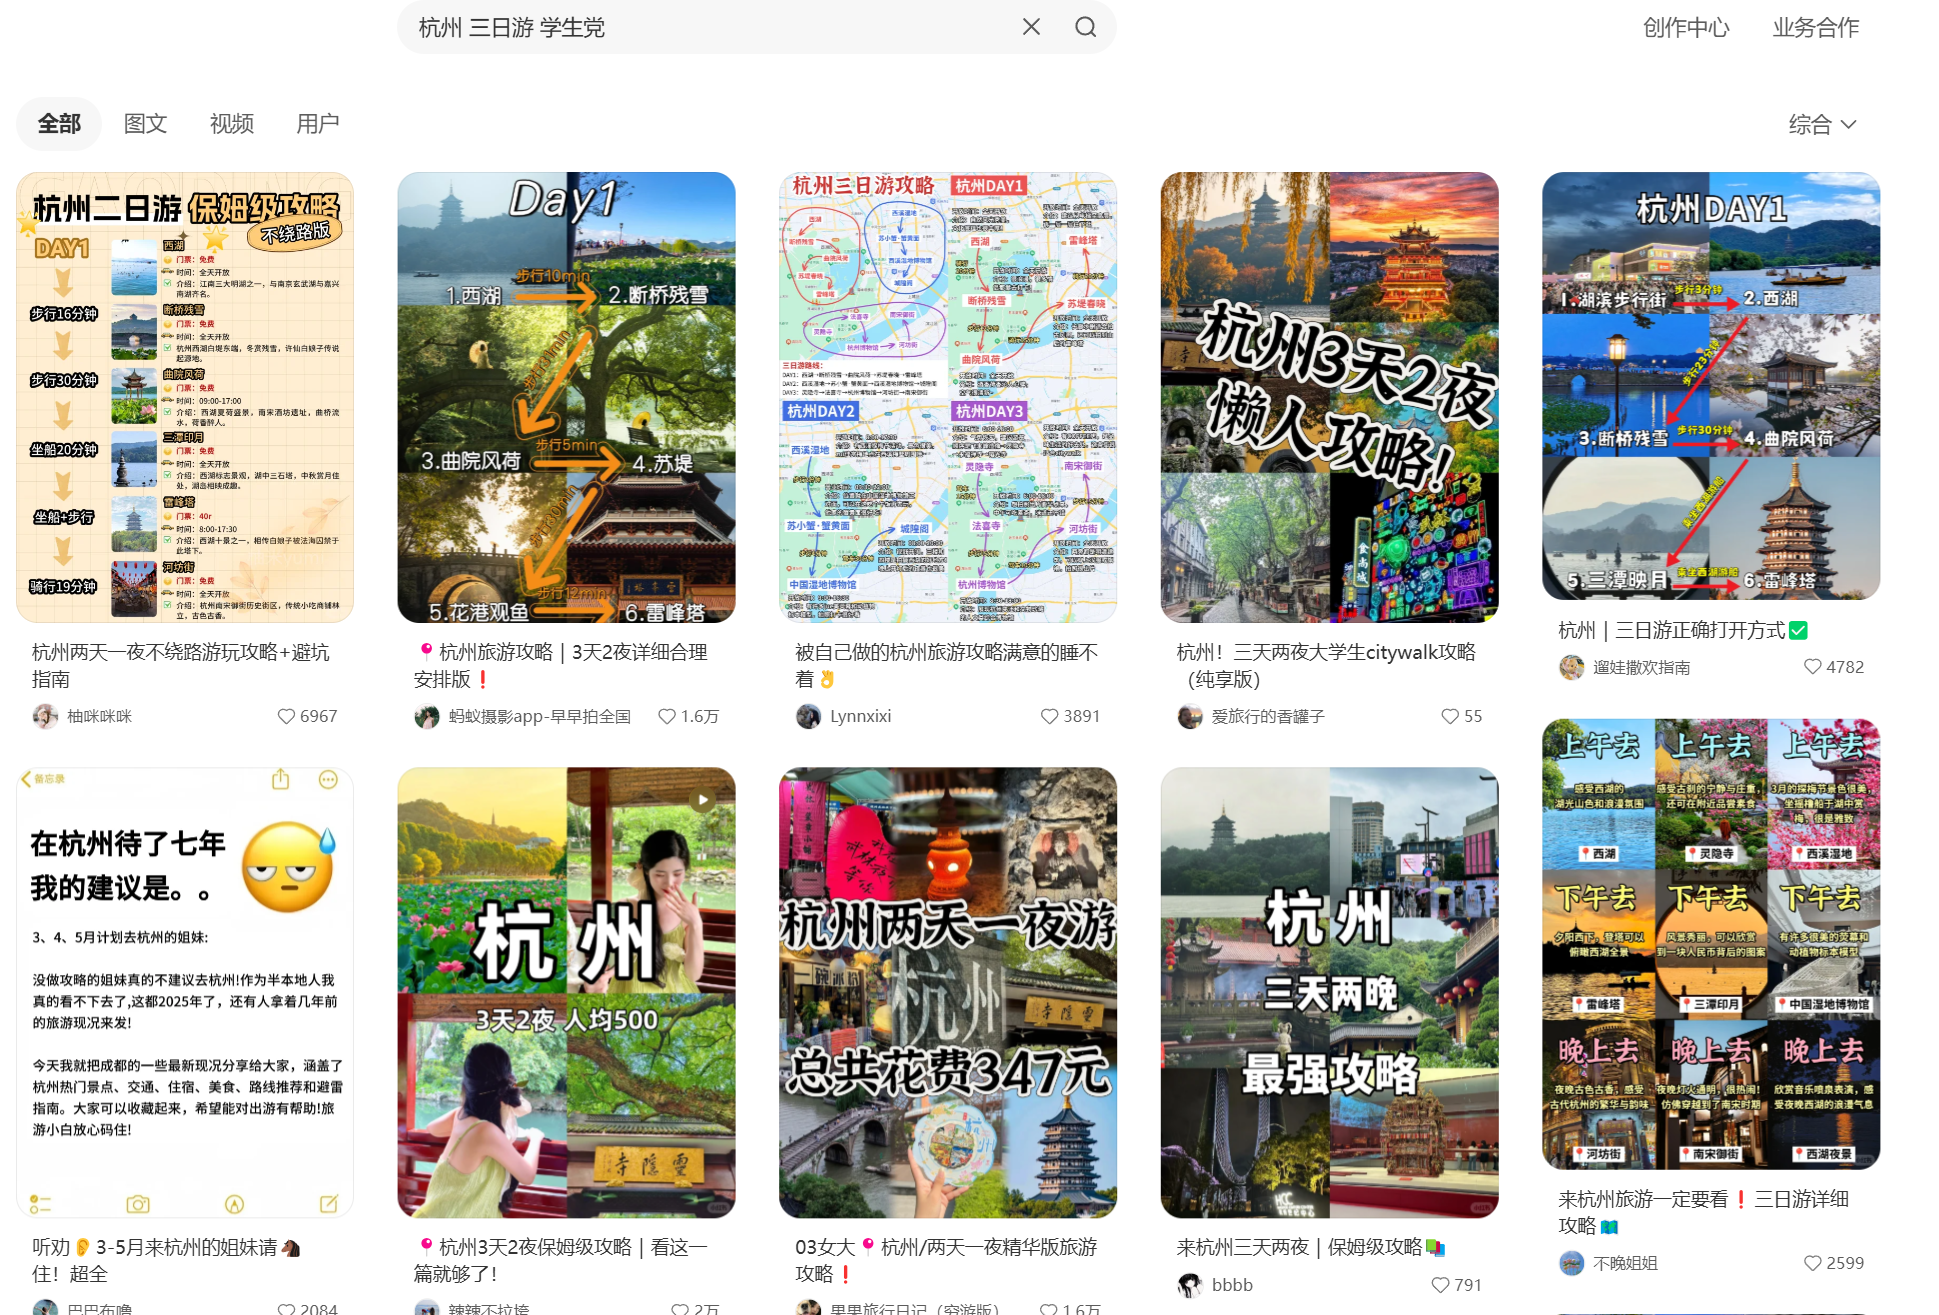
\includegraphics[width=.8\textwidth]{./figures/生活/示例1.png}
\caption{搜索示例}
\end{figure}
\subsection{搜索技巧}
\begin{enumerate}
  \item 关键词组合:如“杭州 三日游 学生党”,“重庆 美食打卡 5月”
  \item 避坑话术:如“XX景点 不要去”
  \item 筛选条件:优先选择“最新发布”“高赞笔记”等,避开广告软文
\end{enumerate}
\subsection{进阶搜索技巧}
\begin{enumerate}
  \item 双引号“”  :强制完全匹配短语,避免拆分或谐音干扰
  \item 减号-    :排除含特定关键词的页面,适用于过滤广告或无关内容。
  \item 通用支持:""、-、site:、filetype:、inurl:、intitle: 等指令适用于Google、Bing、百度等主流搜索引擎。
  \item 部分支持:allintitle:在百度中可能失效,建议拆分为intitle:多关键词组合使用。
\end{enumerate}
\begin{figure}[H]
  \centering
  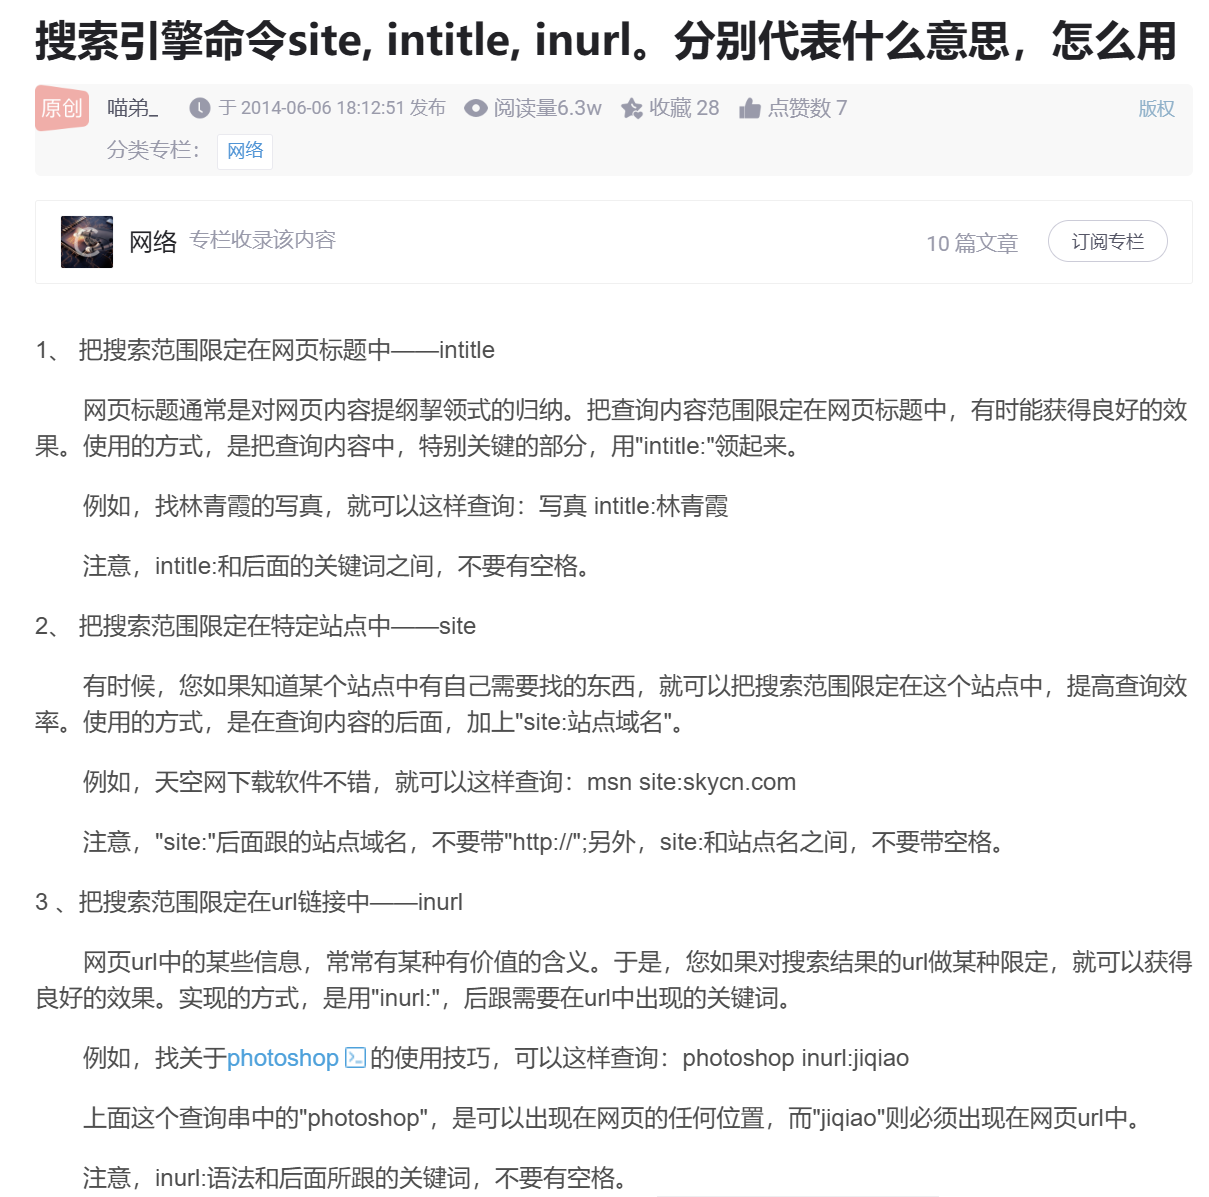
\includegraphics[width=.8\textwidth]{./figures/生活/示例2.png}
  \caption{搜索进阶}
\end{figure}
\begin{exbox}{进阶搜索实例}{advanced search}
  \begin{itemize}
    \item "迪士尼门票折扣" -广告 -推广 intext:2025

    \item intitle:"西湖 醋鱼" intitle:老字号

    \item 限定网站:关键词 site:网站域名(排除非垂直平台信息,提升可信度):如“重庆火锅 site:dianping.com”
  \end{itemize}
\end{exbox}
\subsection{学生特惠}
\begin{enumerate}
  \item 支付宝
  \begin{enumerate}
    \item 校园派:集中展示学生专属红包、任务奖励、品牌联名优惠(如餐饮折扣、出行券包)
    \item 学生特惠:长期展示学生专属折扣商品、生活服务优惠。
  \end{enumerate}
  \begin{figure}[H]
    \centering
    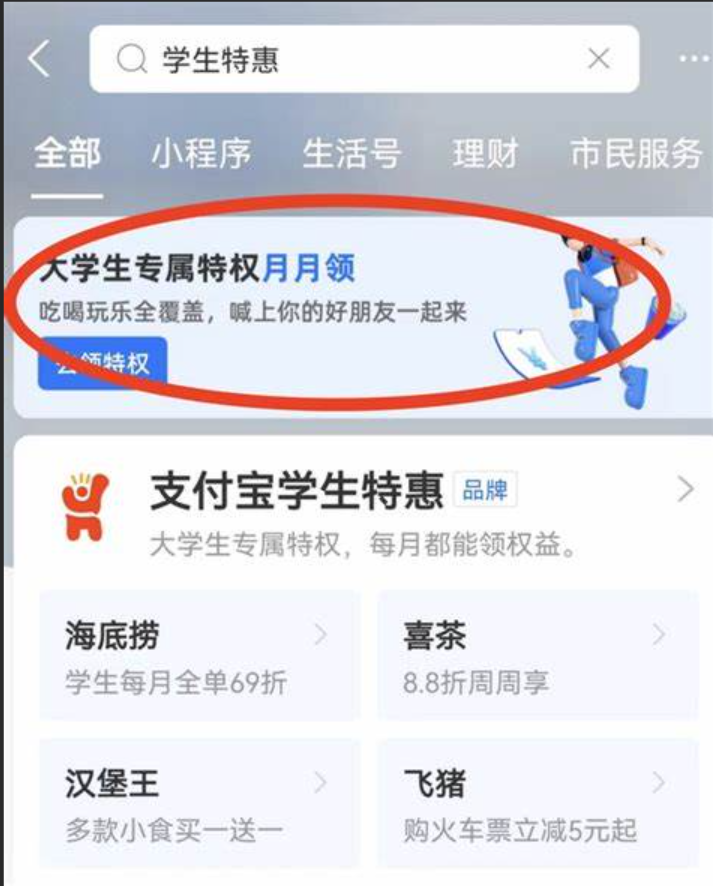
\includegraphics[width=.8\textwidth]{./figures/生活/学生优惠_支付宝.png}
    \caption{支付宝学生优惠}
  \end{figure}
  \item 12306
  \begin{enumerate}
    \item 票价优惠
  \end{enumerate}
  \begin{figure}[H]
    \centering
    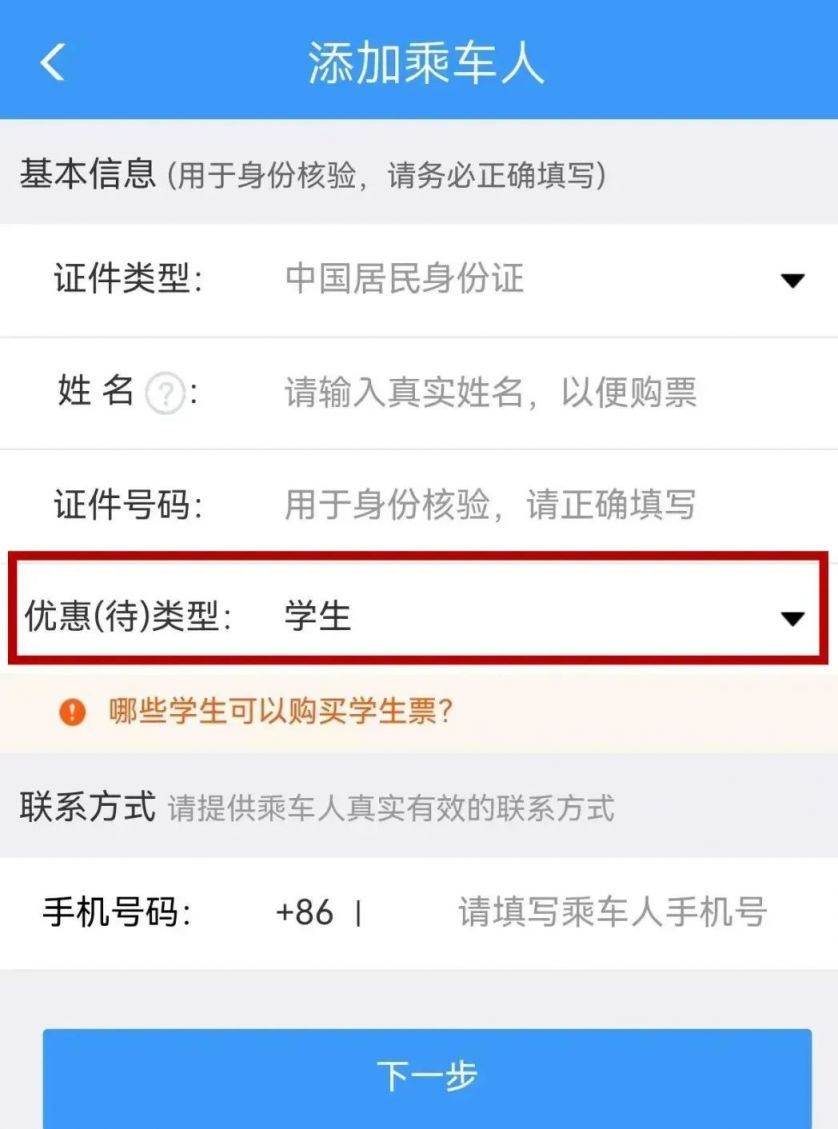
\includegraphics[width=.8\textwidth]{./figures/生活/学生优惠_12306.jpg}
    \caption{12306学生优惠}
  \end{figure}
  \item 美团
  \begin{enumerate}
    \item 学生专属红包/神券
    \item 返校优惠/交通票务折扣
    \item 学生价/首单优惠
  \end{enumerate}
\end{enumerate}
\section{餐饮信息收集}
\subsection{搜索平台}
\begin{enumerate}
  \item 外卖平台(查看商家评分、用户评价、优惠活动):美团、饿了么
  \item 生活平台(筛选“高校周边”“学生推荐”标签):大众点评
\end{enumerate}
\subsection{搜索技巧}
\begin{enumerate}
  \item 关键词组合:「口味+价格」,「品牌+活动」等
  \item 筛选条件:筛选距离,好评,价格区间,用餐场景等等
\end{enumerate}
\textbf{餐饮类重点关注:卫生情况,口味评价,口碑评分等}
\subsection{卫生情况}
\begin{enumerate}
  \item 查看证照信息(操作路径:商家页面 → 资质公示 → 食品经营许可证 )

  在商家页面进入「商家信息」或「资质」板块,重点查看公示的食品经营许可证。持有该证照的商家通常具备固定营业场所,

  \item 查看卫生评级

  部分城市在美团平台标注商家卫生评级(如A/B/C级),优先选择A级或B级商家,此类商家卫生状况更可靠。

  \item 观察环境图片

  商家页面展示的店铺实景图可直观反映堂食环境。若图片包含桌椅、用餐区等元素,则说明支持堂食;若仅展示后厨或打包区,可能为纯外卖店铺。

  \item 分析用户差评

  重点筛选差评中的卫生相关关键词,如“吃出异物”“蟑螂”“油污”“食材不新鲜”等。若差评集中反映卫生问题,需谨慎选择。

\end{enumerate}
\subsection{口碑评分}
\begin{enumerate}
  \item 查看综合评分

  商家页面顶部显示星星数量评分,星星越多代表综合口碑越好。评分基于口味、环境、服务、配送等多维度计算。

  \item  筛选用户评价标签(操作路径:评价区域 → 筛选 → 选择标签类型 )

  在评价区域,可通过筛选功能查看好评、差评或有图评价。美团还提供标签化分类,如“味道赞”“分量足”“服务好”等,快速定位高频评价点

 \item  分析评价内容

  \begin{enumerate}
    \item 好评参考:关注用户对菜品口味、服务态度、环境舒适度的具体描述。
    \item 差评警惕:若差评集中在菜品质量、卫生问题或服务态度,需结合其他信息综合判断。
  \end{enumerate}
\end{enumerate}
\section{娱乐场所信息收集}
\subsection{搜索平台}
\begin{enumerate}
  \item 娱乐类平台(查询演出、电影、展览信息):猫眼、大麦
  \item 生活平台(查看KTV、台球馆、密室逃脱评分) :美团、大众点评
  \item 校园社群(获取学长学姐推荐的“宝藏店铺”):校园墙/朵朵校友圈
\end{enumerate}
\textbf{娱乐场所类重点关注:安全情况,卫生情况,体验情况等}
\subsection{评估安全性}
\begin{enumerate}
  \item 官方在线查询平台
  \begin{enumerate}
    \item 国家企业信用信息公示系统

    查询方式:登录系统官网,输入场所名称或统一社会信用代码,即可获取企业登记信息,包括营业执照状态、经营范围、法定代表人等。

    \item 地方政务服务平台

    查询方式:部分地区提供本地化查询服务(如北京通APP的“娱乐场所营业资格查询”功能),可结合企业信用信息公示系统使用。
  \end{enumerate}
 \item 实地核查
 \begin{enumerate}
  \item 显性标识检查
  \begin{itemize}
    \item 法律依据:根据《中华人民共和国公司法》,营业执照正本应置于经营场所醒目位置。
    \item 操作要点:尽量选择连锁品牌,直接前往场所,查看是否在显眼位置悬挂营业执照,并核对信息是否与场所名称、地址一致。
  \end{itemize}
  \item 证照公示情况

  除营业执照外,娱乐场所还需公示《娱乐经营许可证》等专项许可文件。若场所无法提供或公示信息不完整,可能存在违规经营风险。
 \end{enumerate}
 \item 官方渠道核实

 工商行政管理部门/文化市场监管部门咨询核查

 拨打当地工商部门或文化市场监管部门咨询电话,或前往办事窗口,提供场所名称、地址等信息,申请查询其证照核发和年检状态。

 \item 第三方数据平台

 \begin{enumerate}
  \item 企查查/天眼查

  输入场所名称,查看其关联风险(如行政处罚记录、司法诉讼),曾因不达标/不合规被罚款的场所可能存在安全隐患。
  \item 消费投诉平台
         \begin{itemize}
          \item 12315平台:查询场所投诉量及解决率,高频投诉问题(如“强制消费”“中途加价”)需重点警惕。
          \item 黑猫投诉:搜索场所名称,关注用户上传的交易凭证(如消费小票、聊天记录)
         \end{itemize}
 \end{enumerate}
\end{enumerate}
\subsection{卫生情况}
\begin{enumerate}
  \item 公示文件核查:查看场所是否悬挂《公共场所卫生许可证》,有效期通常为4年,需确认是否在有效期内。
  \item 环境细节观察:
         \begin{enumerate}
          \item 包厢清洁:桌面、地面无杂物水渍,沙发/皮凳无污渍,踢脚板无灰尘。
          \item 设备卫生:麦克风球套定期更换,麦克风头无损坏,点歌面板无灰尘。
          \item 公共区域:卫生间面盆、浴缸、坐便器每客一消毒,无积水、污垢或异味;垃圾桶及时清倒,垃圾袋及时更换
         \end{enumerate}
  \item 卫生等级参考
        \begin{enumerate}
          \item \item 部分地区对娱乐场所进行卫生评级(如A级优秀、B级良好、C级一般),可通过当地卫生监督部门官网查询场所评级信息。  3. 卫生检测报告
         \item 正规场所应定期进行空气质量、水质、噪声等检测,并公示检测报告。可要求场所提供近期检测报告,重点关注甲醛、二氧化碳、细菌总数等指标是否达标。
        \end{enumerate}
\end{enumerate}
\subsection{口碑情况}
\begin{enumerate}
  \item 主流消费平台
  \begin{enumerate}
    \item 美团/大众点评:

    通过搜索KTV名称查看综合评分(满分5分)及用户评价标签(如“音效好”“服务热情”)。

    重点关注高频差评关键词,如“设备故障”“服务冷漠” “曲库更新”“隔音效果”“包厢卫生”等,可直观反映实际体验。
    \item 带图评价:用户上传的包厢环境、设备状态等照片,可辅助判断场所条件。
  \end{enumerate}

  \item 垂直领域平台
        \begin{enumerate}
          \item 小红书/抖音/哔哩哔哩:关注博主探店视频中的音效测试、卫生细节、套餐性价比分析。
          \item 本地/校园生活论坛:获取居民/朋辈对场所的长期口碑反馈
        \end{enumerate}
  \item 社交媒体舆情监测
  \begin{enumerate}
    \item 微博超话/话题
    \item 微信生态(公众号/朋友圈)
  \end{enumerate}
\end{enumerate}
\section{案例分享}
\begin{exbox}{挑选校园附近KTV}{KTV}
  通过四种途径,展示挑选校园附近KTV的方法
  \tcblower
  \begin{enumerate}
    \item 小红书搜索筛选

    组合关键词搜索+排序标签筛选+评论查看(并关注点赞,收藏数)

    锁定门店候选
    \begin{figure}[H]
      \centering
      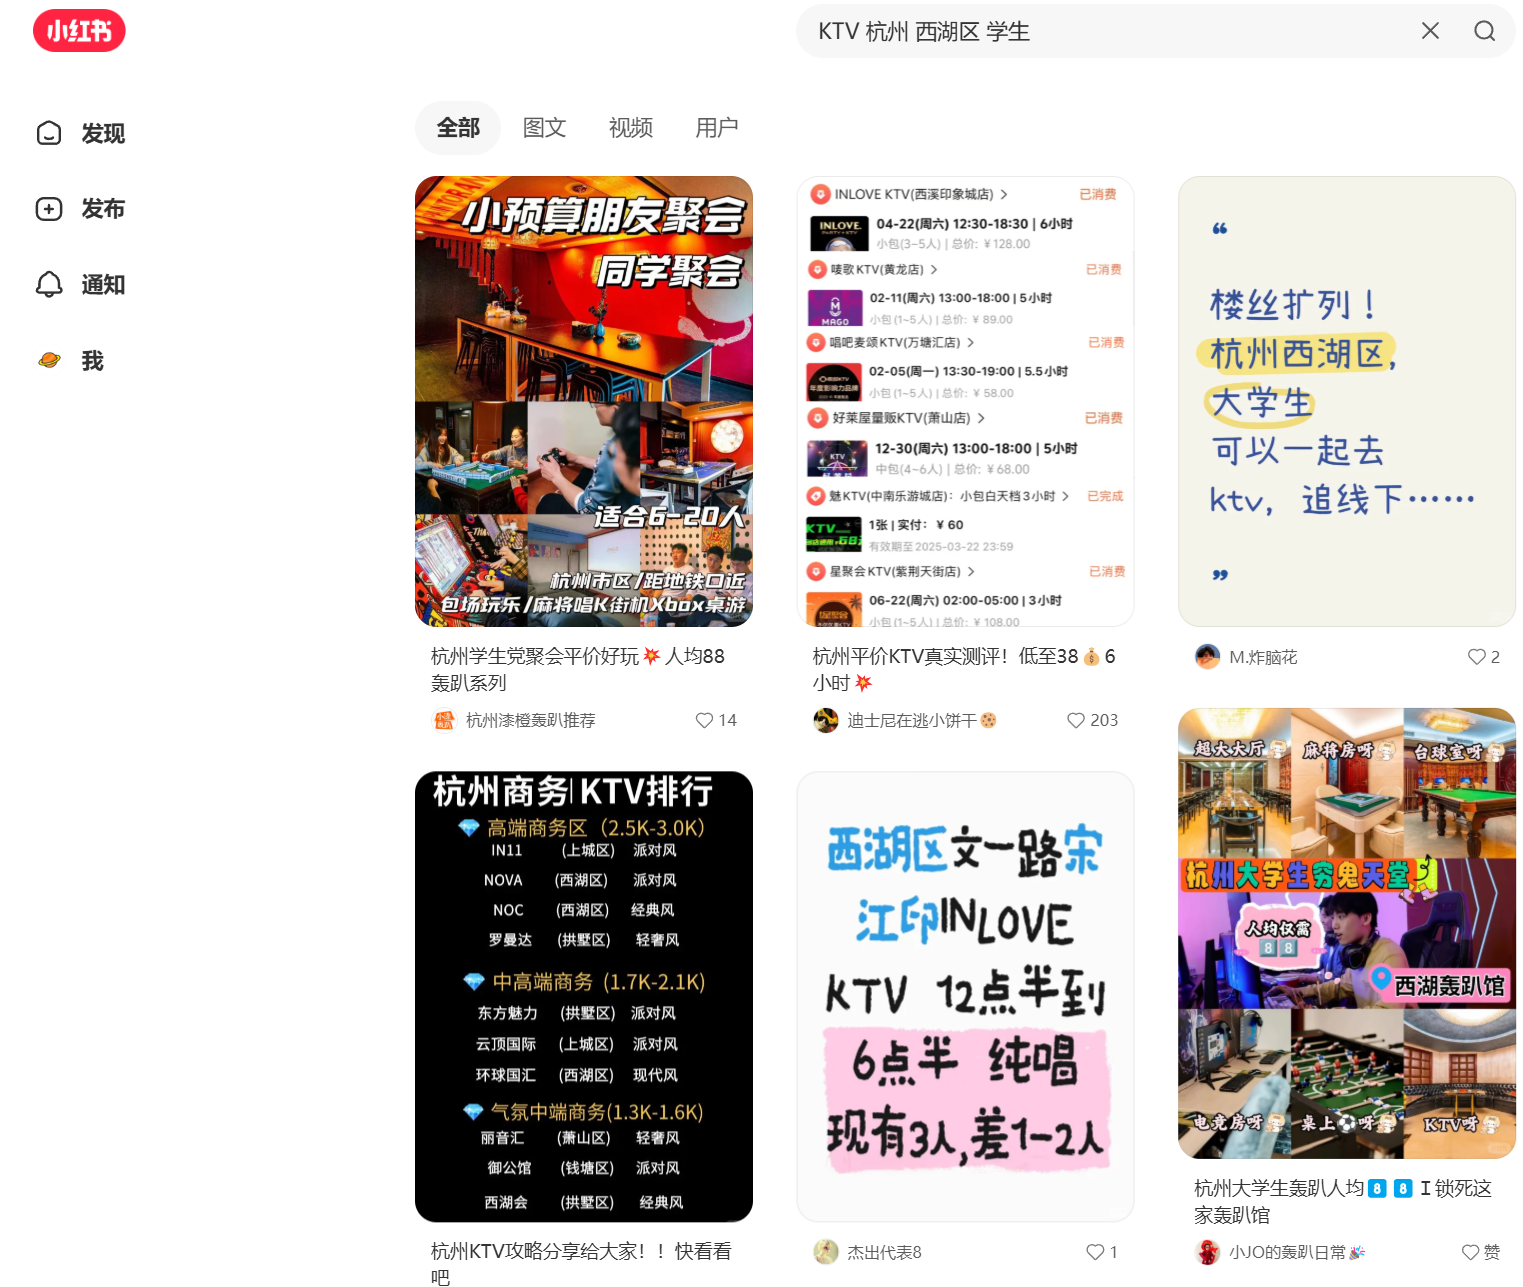
\includegraphics[width=.4\textwidth]{./figures/生活/ktv/1.png}
      \qquad
      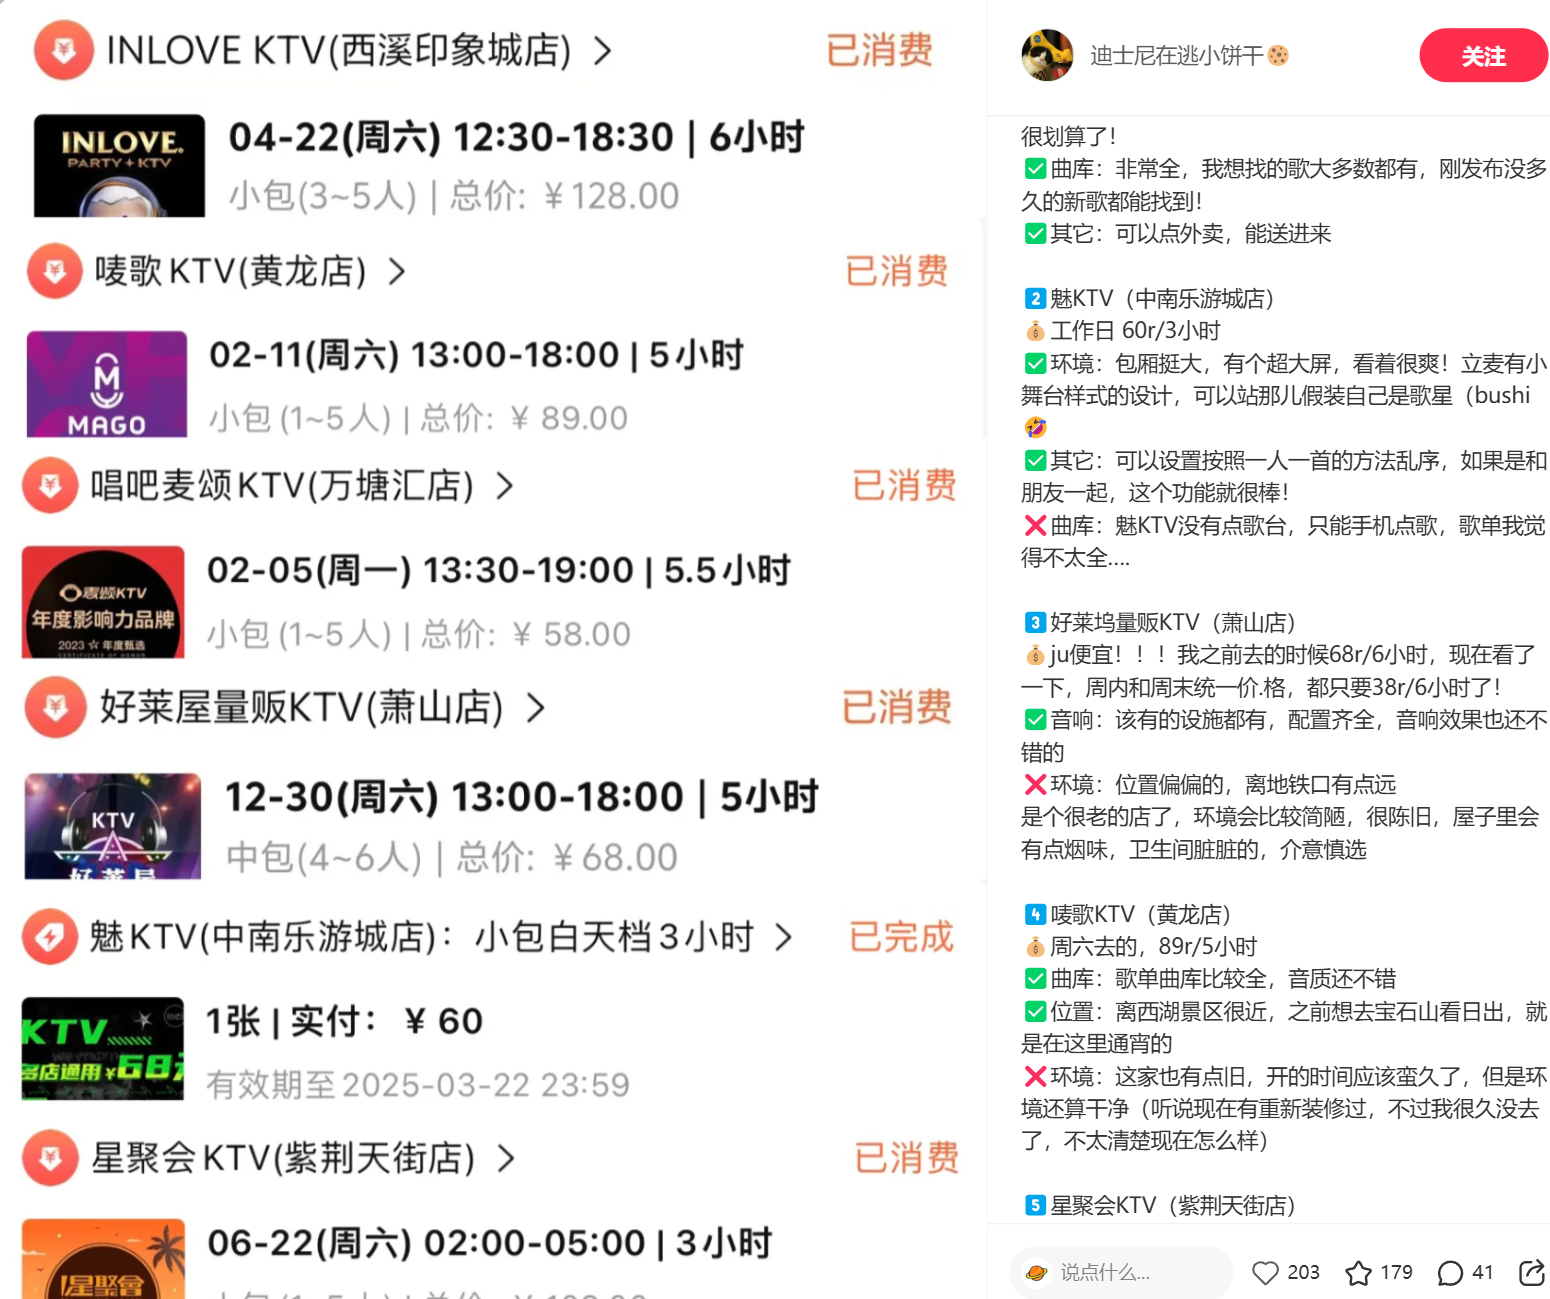
\includegraphics[width=.4\textwidth]{./figures/生活/ktv/2.png}
      \caption{小红书}
    \end{figure}

  \item 哔哩哔哩探店视频

  实景+测评查看(并关注点赞,收藏,转发数)

  寻求好评门店重叠

  \begin{figure}[H]
    \centering
    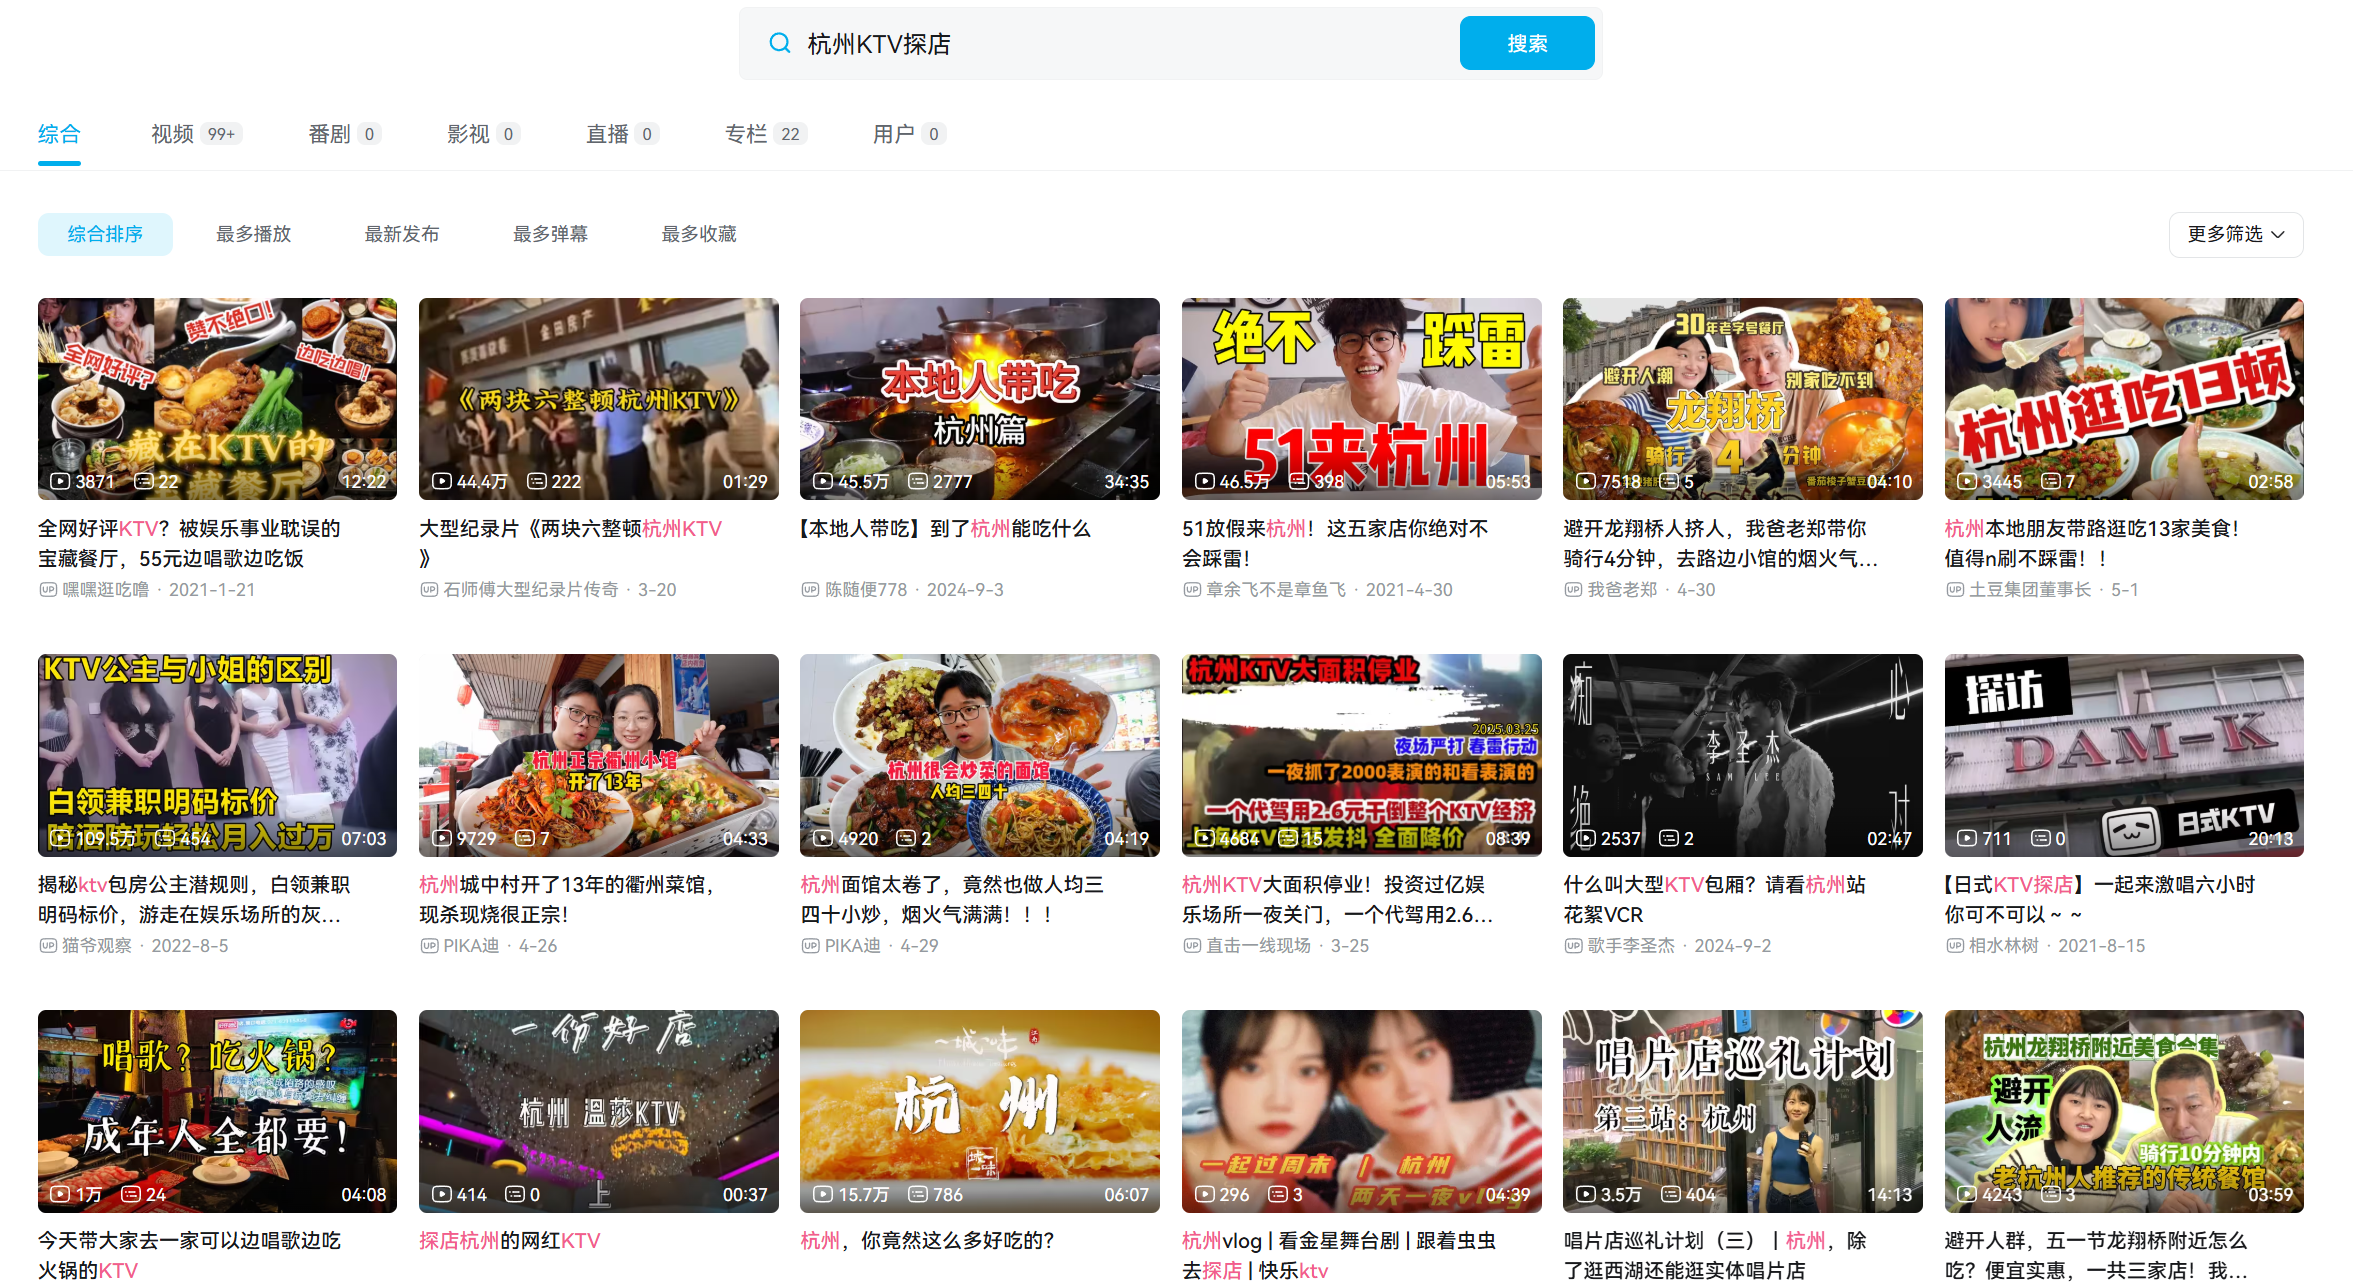
\includegraphics[width=.8\textwidth]{./figures/生活/ktv/bili.png}
    \caption{BiliBili}
  \end{figure}
  \item 美团搜索具体门店

  评分评论(重点关注差评率+差评理由,特别是卫生环境问题)+价格/门店信息查看+经营资质证明查看
  \begin{figure}[H]
    \centering
    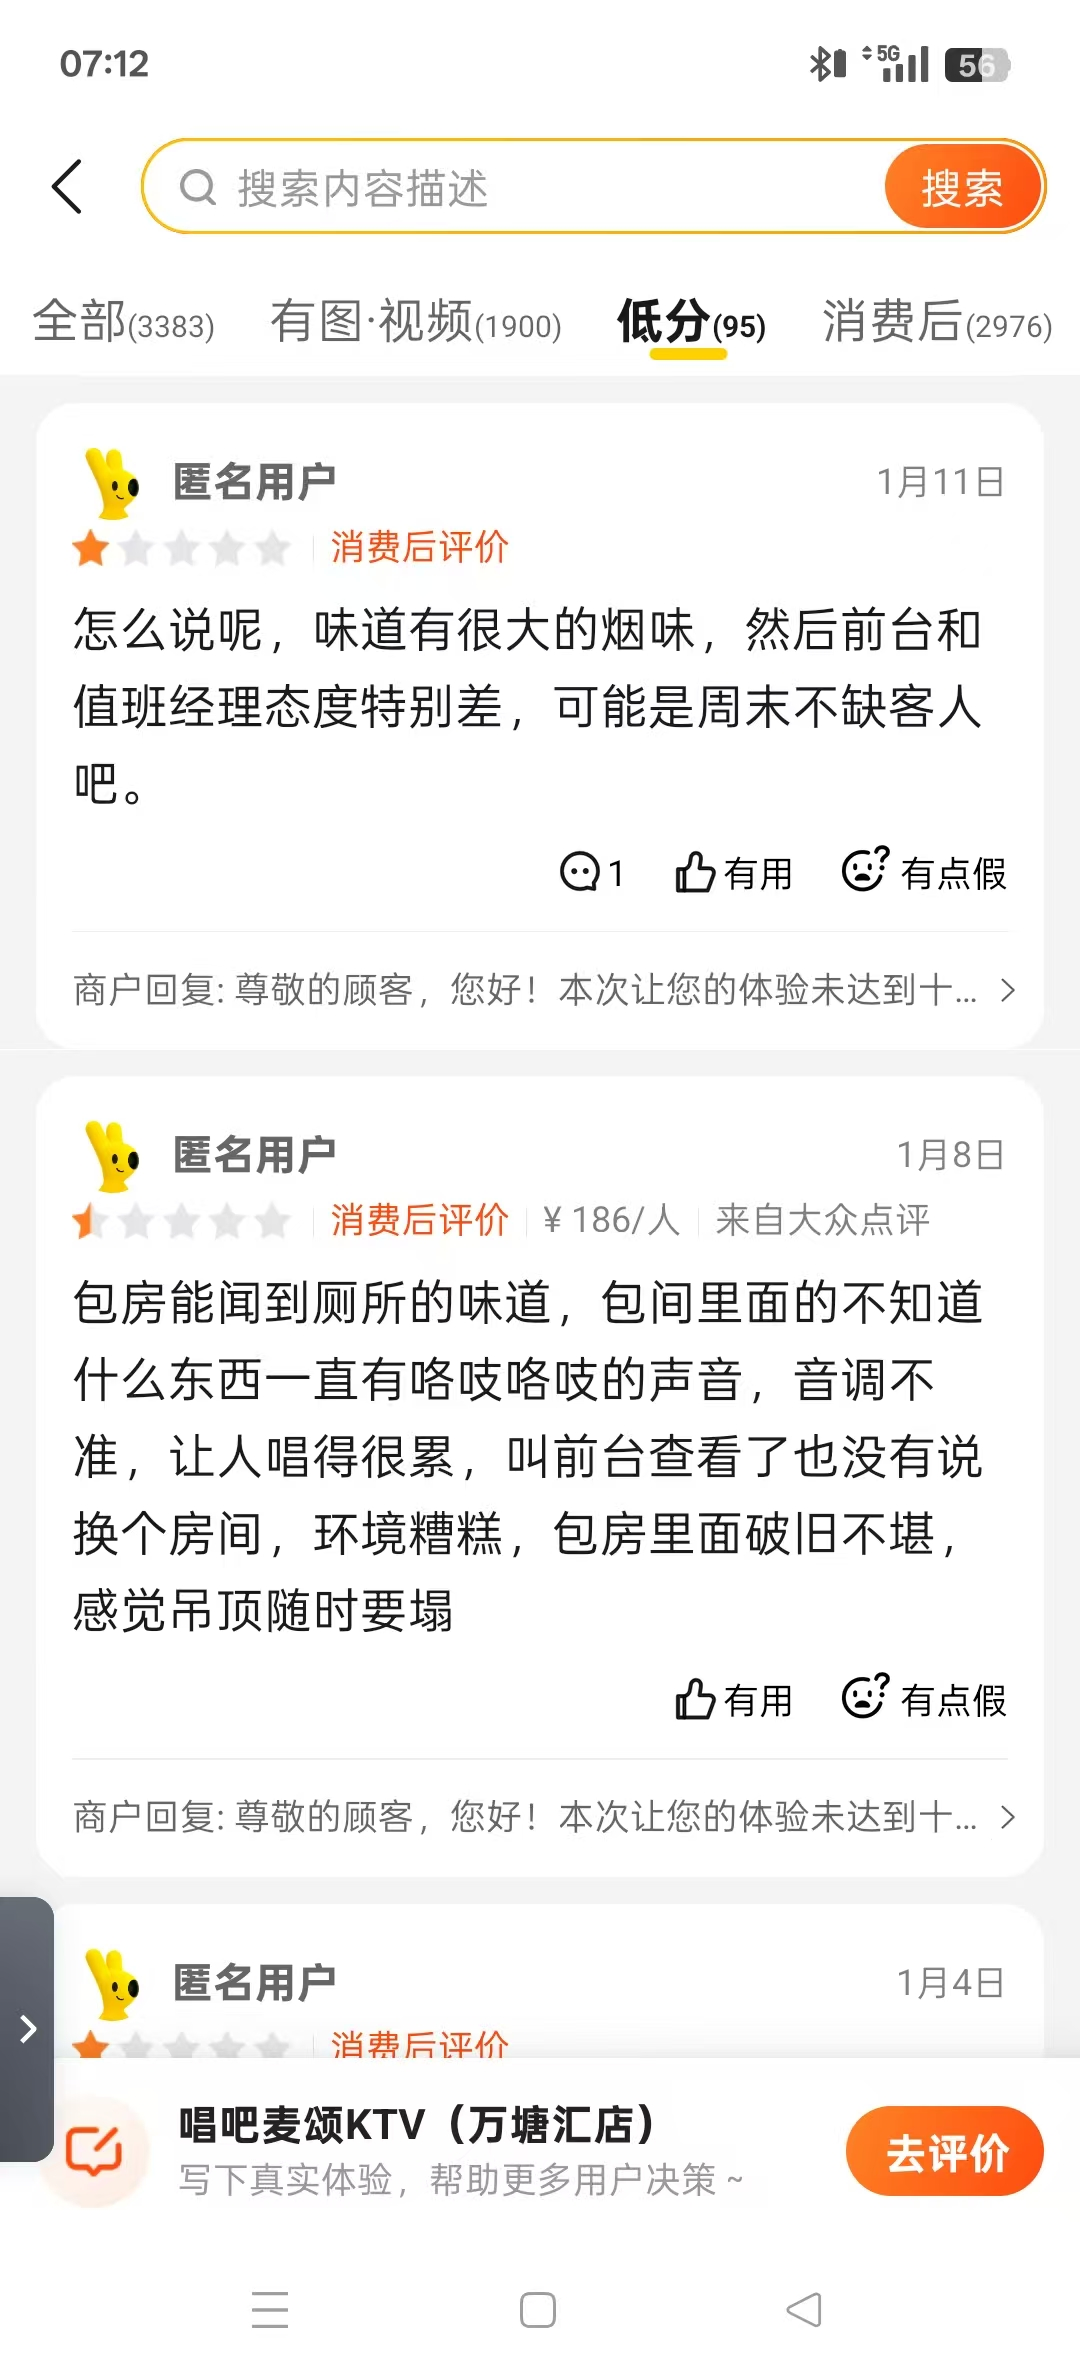
\includegraphics[width=.4\textwidth]{./figures/生活/ktv/m1.jpg}
    \qquad
    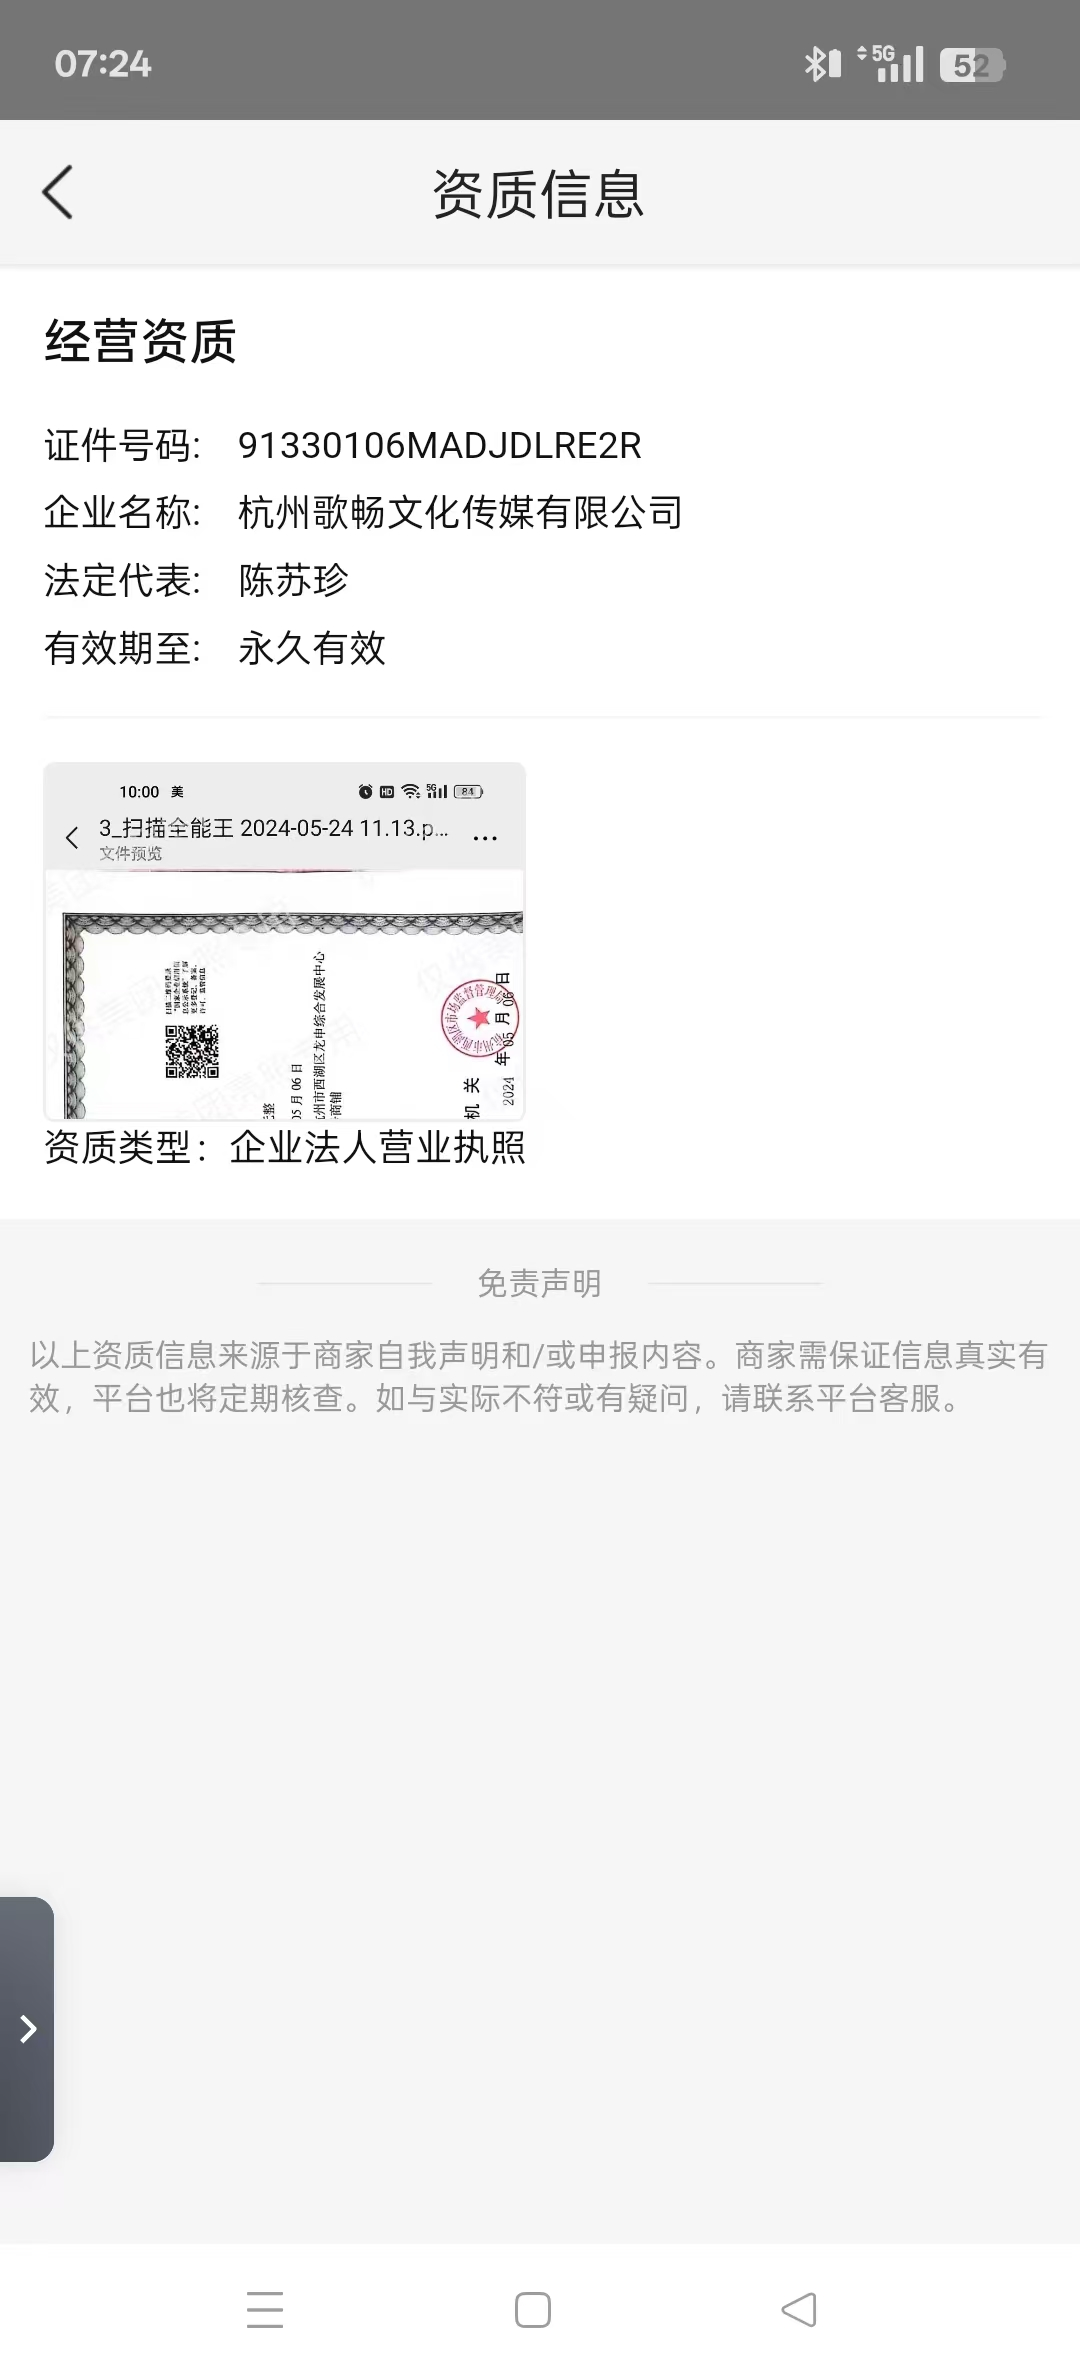
\includegraphics[width=.4\textwidth]{./figures/生活/ktv/m2.jpg}
    \caption{美团}
  \end{figure}
  \item 校友圈搜索相关体验回馈
  \begin{figure}[H]
    \centering
    
\includegraphics[width=.5\textwidth]{./figures/生活/ktv/d1.jpg}
    \caption{朵朵校友圈}
  \end{figure}
  \end{enumerate}
\end{exbox}
\end{document}